%===============================================================
%   Design Documentation
%===============================================================

\documentclass[parskip=full]{scrartcl}

\usepackage{enumerate}
\usepackage[shortlabels]{enumitem}
\usepackage[utf8]{inputenc} % use utf8 file encoding for TeX sources
\usepackage[T1]{fontenc} % avoid garbled Unicode text in pdf
\usepackage{hyperref} % detailed hyperlink/pdf configuration
\usepackage{csquotes} % provides \enquote{} macro for "quotes"
\usepackage{graphicx} % embed graphics
\usepackage[toc]{glossaries}
 
% definitions
\newcommand{\pseProjectName}{An Interactive End-To-End Machine Learning Platform}
\newcommand{\pseTitle}{\pseProjectName}
\newcommand{\pseDocTitle}{Design}

\hypersetup{ % ‘texdoc hyperref‘ for options
pdftitle={\pseDocTitle}}
\title{%
    \pseTitle \\
    \large \pseDocTitle
    \date{\today}
}
\makenoidxglossaries
\loadglsentries{glossary}
\begin{document}

\begin{titlepage}
    \maketitle
    \begin{center}
        \begin{tabular}{ r l }
            Requirements Specification & \textbf{Murat Kurnaz}         \\
            Design                     & \textbf{Mustafa Enes Batur}   \\
            Implementation             & \textbf{Ömer Erdinç Yağmurlu} \\
            QA / Testing               & \textbf{Tarek Gaddour}        \\
            Final                      & \textbf{Atalay Donat}         \\
        \end{tabular}
    \end{center}
\end{titlepage}

\tableofcontents

\section{Introduction}
The purpose of this documentation is to inform the reader about the design of our project. For this purpose readers are presented with class and sequence diagrams. Class diagrams show the general hierarchy and relation between the classes. Seqeunce diagrams are used to provide the reader an intuition about how different classes interact with each other during runtime of the software.
\newpage
\section{Structure}

\subsection{Architecture}
\begin{figure}[hb]
    \centering
    \fbox{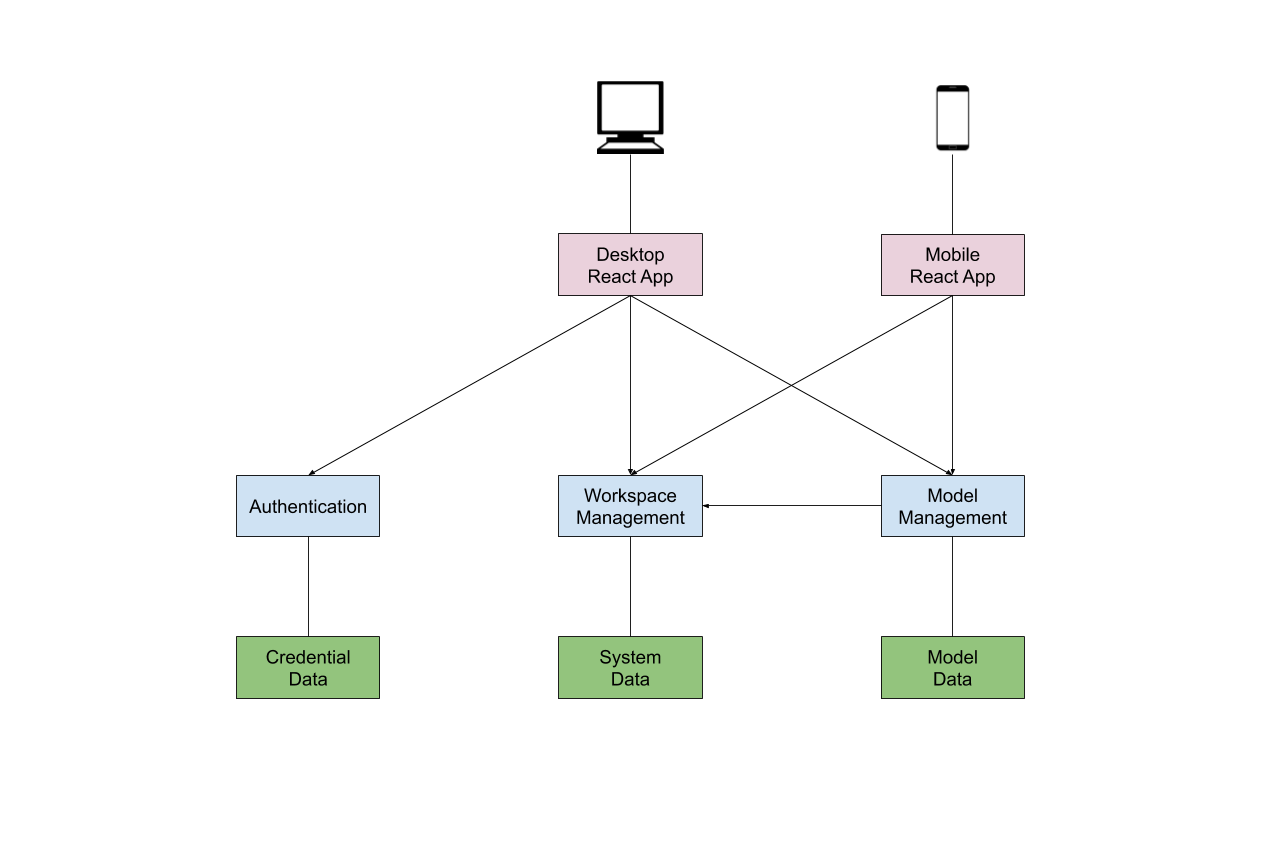
\includegraphics[width = .98\textwidth]{figures/architecture.png}}
    \caption{System Architecture as Microservices}
    \label{fig:microservices}
\end{figure}

General system architecture is designed according to the microservices architecture. Details of each microservice can be found below.

\subsection{Authentication}
Authentication service handles the registration of new users and authentication of registered users. The user registers by choosing a username, a password and supplying his email address. The authentication service then sends a verification token to this email address. The user creation is completed after the email verification.
\par The service uses JSON Web Tokens as the authentication method. After logging in, the user receives a cryptographically encrypted access token which is saved as a cookie. We encrypt the JWT that includes the username of the user and an expiration time (15 minutes after the creation) with a secret phrase that is shared among all the services that wish to use authentication. After receiving the access token with the requests, the services are able to decrypt the access token and verify the user identity. The user receives a refresh token in addition to the access token. This refresh token is used to renew an expired access token. This way, the user does not need to enter his credentials each time the token expires.

\subsection{Workspace Management}
Workspace Management Service manages the workspaces of the system. When the user creates a workspace, a database entry corresponding to that workspace is created in this service. All the data that is needed for data collection and storage of a workspace, i.e. the sensors that are used in the workspace, the labels that the user created and the samples that were collected, are stored in the database of this service. Workspace Management serves an endpoint to receive raw sensor data for each workspace and stores the data without any processing. It serves the collected data to the Model Management service for processing and model training purposes. The server runs on Node.js and uses MongoDB to store its data. In short, the service creates an interface between the database and the client.

\subsection{Mobile and Desktop Clients}
Clients are implemented in a client-side-routed web app fashion using React and a routing library called raviger. All communication is routed through the API class, which, alongside dealing with authentication, acts as an adapter to the backend.


\newpage
\section{Class Description}

\subsection{Authentication}
\subsubsection{App}
\label{App}
\begin{wrapfigure}{l}{4.5cm}
    \raisebox{0pt}[\dimexpr\height-0.5\baselineskip\relax]{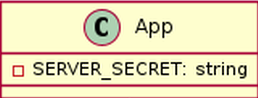
\includegraphics[width=4.5cm]{classes/auth/app.png}}
\end{wrapfigure} 
\par
The main class of the authentication service.
\newline
\newline
\textbf{Attributes}
\begin{itemize}
    \item \textbf{SERVER\_SECRET} the encryption key that is shared among all the services to decrypt tokens
\end{itemize}

\subsubsection{UserModel}
\label{UserModel}
\begin{wrapfigure}{l}{4.5cm}
    \raisebox{0pt}[\dimexpr\height-0.5\baselineskip\relax]{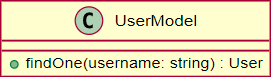
\includegraphics[width=4.5cm]{classes/auth/1.png}}
\end{wrapfigure} 
\par
The collection of registered users in the database.
\newline
\newline
\textbf{Methods}
\begin{itemize}
    \item \textbf{findOne} returns the user that has the matching username
\end{itemize}

\subsubsection{User}
\label{User}
\begin{wrapfigure}{l}{4.5cm}
    \raisebox{0pt}[\dimexpr\height-0.5\baselineskip\relax]{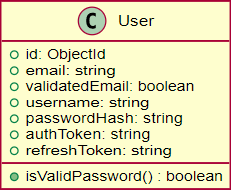
\includegraphics[width=4.5cm]{classes/auth/2.png}}
\end{wrapfigure} 
\par
A registered user
\newline
\newline
\textbf{Attributes}
\begin{itemize}
    \item \textbf{email} email of the user
    \item \textbf{validatedEmail} iff the email is validated
    \item \textbf{username} username of the user
    \item \textbf{passwordHash} hash of the password of the user
    \item \textbf{authToken} the current authentication token of the user
    \item \textbf{refreshToken} the current refresh token of the user
\end{itemize}
\textbf{Methods}
\begin{itemize}
    \item \textbf{isValidPassword} iff the supplied password is valid
\end{itemize}

\subsubsection{EmailValidator}
\label{EmailValidator}
\begin{wrapfigure}{l}{4.5cm}
    \raisebox{0pt}[\dimexpr\height-0.5\baselineskip\relax]{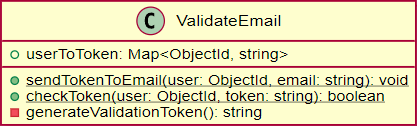
\includegraphics[width=4.5cm]{classes/auth/3.png}}
\end{wrapfigure} 
\par
This static class sends an email to the user with a token and checks if the given token is correct.
\newline
\newline
\textbf{Attributes}
\begin{itemize}
    \item \textbf{userToToken} maps the user id to the sent token
\end{itemize}
\textbf{Methods}
\begin{itemize}
    \item \textbf{sendTokenToEmail} sends a token to the given email 
    \item \textbf{checkToken} compares the received token with the token sent to email
    \item \textbf{generateValidationToken} generates a validation token
\end{itemize}

\subsubsection{TokenContent}
\label{TokenContent}
\begin{wrapfigure}{l}{4.5cm}
    \raisebox{0pt}[\dimexpr\height-0.5\baselineskip\relax]{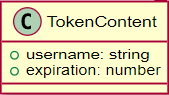
\includegraphics[width=4.5cm]{classes/auth/4.png}}
\end{wrapfigure} 
\par
This class depicts a unencrypted access token.
\newline
\newline
\textbf{Attributes}
\begin{itemize}
    \item \textbf{username} username of the owner of the token
    \item \textbf{expiration} expiration time of the token
\end{itemize}

\subsection{Workspace Management}

\subsubsection{WorkspaceModel}
\label{WorkspaceModel}
\begin{wrapfigure}{l}{4.5cm}
    \raisebox{0pt}[\dimexpr\height-0.5\baselineskip\relax]{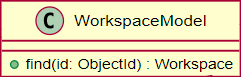
\includegraphics[width=4.5cm]{classes/workspace-management/1.png}}
\end{wrapfigure} 
\par
The collection of workspaces in the database.
\newline
\newline
\textbf{Methods}
\begin{itemize}
    \item \textbf{find} returns the workspace with the given ID.
\end{itemize}

\subsubsection{Workspace}
\label{wm-Workspace}
\begin{wrapfigure}{l}{4.5cm}
    \raisebox{0pt}[\dimexpr\height-0.5\baselineskip\relax]{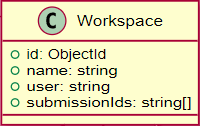
\includegraphics[width=4.5cm]{classes/workspace-management/2.png}}
\end{wrapfigure} 
\par
The document that includes all the relevant information about a workspace.
\newline
\newline
\textbf{Attributes}
\begin{itemize}
    \item \textbf{name} name of the workspace
    \item \textbf{user} user of the workspace
    \item \textbf{submissionIds} all valid submission IDs of the workspace
\end{itemize}

\subsubsection{SensorType}
\label{SensorType}
\begin{wrapfigure}{l}{4.5cm}
    \raisebox{0pt}[\dimexpr\height-0.5\baselineskip\relax]{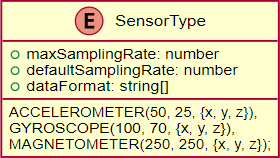
\includegraphics[width=4.5cm]{classes/workspace-management/4.png}}
\end{wrapfigure} 
\par
This enumeration consists of the supported sensors.
\newline
\newline
\textbf{Attributes}
\begin{itemize}
    \item \textbf{maxSamplingRate} the maximum sampling rate of the sensor
    \item \textbf{defaultSamplingRate} the default sampling rate of the sensor
    \item \textbf{dataFormat} the data format of the sensor
\end{itemize}

\subsubsection{Sensor}
\label{Sensor}
\begin{wrapfigure}{l}{4.5cm}
    \raisebox{0pt}[\dimexpr\height-0.5\baselineskip\relax]{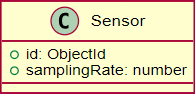
\includegraphics[width=4.5cm]{classes/workspace-management/3.png}}
\end{wrapfigure} 
\par
This class represents a chosen sensor of the workspace. 
\newline
\newline

\textbf{Attributes}
\begin{itemize}
    \item \textbf{samplingRate} the selected sampling rate of the sensor
\end{itemize}

\subsubsection{Label}
\label{Label}
\begin{wrapfigure}{l}{4.5cm}
    \raisebox{0pt}[\dimexpr\height-0.5\baselineskip\relax]{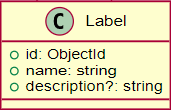
\includegraphics[width=4.5cm]{classes/workspace-management/5.png}}
\end{wrapfigure} 
\par
This class represent an action that describes a sample.
\newline
\newline
\textbf{Attributes}
\begin{itemize}
    \item \textbf{name} name of the label
    \item \textbf{description} description of the label
\end{itemize}

\subsubsection{SampleModel}
\label{SampleModel}
\begin{wrapfigure}{l}{4.5cm}
    \raisebox{0pt}[\dimexpr\height-0.5\baselineskip\relax]{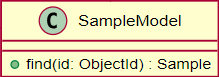
\includegraphics[width=4.5cm]{classes/workspace-management/6.png}}
\end{wrapfigure} 
\par
The collection of samples in the database.
\newline
\newline
\textbf{Methods}
\begin{itemize}
    \item \textbf{find} returns the sample with the given ID.
\end{itemize}

\subsubsection{Sample}
\label{Sample}
\begin{wrapfigure}{l}{4.5cm}
    \raisebox{0pt}[\dimexpr\height-0.5\baselineskip\relax]{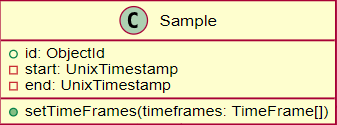
\includegraphics[width=4.5cm]{classes/workspace-management/7.png}}
\end{wrapfigure} 
\par
This class represents a document in the database that contains raw sensor data, its selected timeframes and its label.
\newline
\newline
\textbf{Attributes}
\begin{itemize}
    \item \textbf{start} the timestamp of the start of recording
    \item \textbf{end} the timestamp of the end of recording
\end{itemize}
\textbf{Methods}
\begin{itemize}
    \item \textbf{setTimeFrames} sets the timeframes of the sample
\end{itemize}

\subsubsection{SensorDataPoints}
\label{SensorDataPoints}
\begin{wrapfigure}{l}{4.5cm}
    \raisebox{0pt}[\dimexpr\height-0.5\baselineskip\relax]{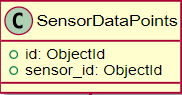
\includegraphics[width=4.5cm]{classes/workspace-management/8.png}}
\end{wrapfigure} 
\par
This class represents data points of a specific sensor.
\newline
\newline
\textbf{Attributes}
\begin{itemize}
    \item \textbf{sensor\_id} the ID of the sensor to which the data belongs
\end{itemize}

\subsubsection{DataPoint}
\label{DataPoint}
\begin{wrapfigure}{l}{4.5cm}
    \raisebox{0pt}[\dimexpr\height-0.5\baselineskip\relax]{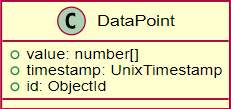
\includegraphics[width=4.5cm]{classes/workspace-management/9.png}}
\end{wrapfigure} 
\par
This class is blablabla and bla bla bla. This denotes bla bla bla and provided by Selehaddin Ozdemir. xdaslkads anu adl kl;asd k;lads l;l;kasdk ;lkdsa;k lllld kksdk mjdask hdaksjhd haso sadjh salk da.
\newline
\newline
\textbf{Attributes}
\begin{itemize}
    \item \textbf{value}
    \item \textbf{timestamp}
\end{itemize}

\subsubsection{TimeFrame}
\label{TimeFrame}
\begin{wrapfigure}{l}{4.5cm}
    \raisebox{0pt}[\dimexpr\height-0.5\baselineskip\relax]{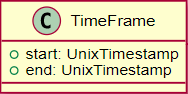
\includegraphics[width=4.5cm]{classes/workspace-management/10.png}}
\end{wrapfigure} 
\par
This class is blablabla and bla bla bla. This denotes bla bla bla and provided by Selehaddin Ozdemir. xdaslkads anu adl kl;asd k;lads l;l;kasdk ;lkdsa;k lllld kksdk mjdask hdaksjhd haso sadjh salk da.
\newline
\newline
\textbf{Attributes}
\begin{itemize}
    \item \textbf{start}
    \item \textbf{end}
\end{itemize}

\subsection{Model Management}

\subsubsection{Trainer}
\label{Trainer}
\begin{wrapfigure}{l}{4.5cm}
    \raisebox{0pt}[\dimexpr\height-0.5\baselineskip\relax]{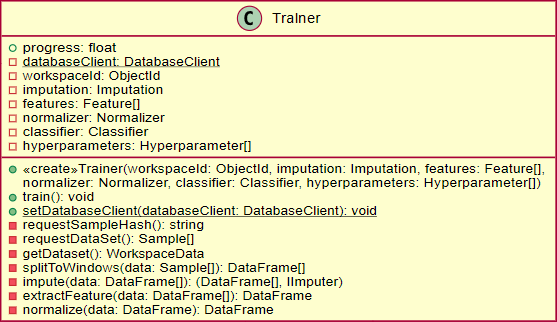
\includegraphics[width=4.5cm]{classes/model-management/1.png}}
\end{wrapfigure} 
\par
This class is blablabla and bla bla bla. This denotes bla bla bla and provided by Selehaddin Ozdemir. xdaslkads anu adl kl;asd k;lads l;l;kasdk ;lkdsa;k lllld kksdk mjdask hdaksjhd haso sadjh salk da.
\newline
\newline
\textbf{Attributes}
\begin{itemize}
    \item \textbf{progress}
    \item \textbf{databaseClient}
    \item \textbf{workspaceId}
    \item \textbf{imputation}
    \item \textbf{features}
    \item \textbf{normalizer}
    \item \textbf{classifier}
    \item \textbf{hyperparameters}
\end{itemize}
\textbf{Methods}
\begin{itemize}
    \item \textbf{train}
    \item \textbf{setDatabaseClient}
    \item \textbf{requestSampleHash}
    \item \textbf{requestDataSet}
    \item \textbf{splitToWindows}
    \item \textbf{impute}
    \item \textbf{extractFeature}
    \item \textbf{normalize}
\end{itemize}

\subsubsection{Workspace}
\label{mm-Workspace}
\begin{wrapfigure}{l}{4.5cm}
    \raisebox{0pt}[\dimexpr\height-0.5\baselineskip\relax]{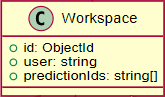
\includegraphics[width=4.5cm]{classes/model-management/2.png}}
\end{wrapfigure} 
\par
This class is blablabla and bla bla bla. This denotes bla bla bla and provided by Selehaddin Ozdemir. xdaslkads anu adl kl;asd k;lads l;l;kasdk ;lkdsa;k lllld kksdk mjdask hdaksjhd haso sadjh salk da.
\newline
\newline
\textbf{Attributes}
\begin{itemize}
    \item \textbf{user}
    \item \textbf{predictionIds}
\end{itemize}

\subsubsection{Sensor}
\label{mm-Sensor}
\begin{wrapfigure}{l}{4.5cm}
    \raisebox{0pt}[\dimexpr\height-0.5\baselineskip\relax]{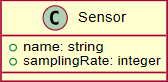
\includegraphics[width=4.5cm]{classes/model-management/3.png}}
\end{wrapfigure} 
\par
This class is blablabla and bla bla bla. This denotes bla bla bla and provided by Selehaddin Ozdemir. xdaslkads anu adl kl;asd k;lads l;l;kasdk ;lkdsa;k lllld kksdk mjdask hdaksjhd haso sadjh salk da.
\newline
\newline
\textbf{Attributes}
\begin{itemize}
    \item textbf{name}
    \item textbf{samplingRate}
\end{itemize}

\subsubsection{MLModel}
\label{MLModel}
\begin{wrapfigure}{l}{4.5cm}
    \raisebox{0pt}[\dimexpr\height-0.5\baselineskip\relax]{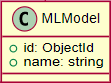
\includegraphics[width=4.5cm]{classes/model-management/4.png}}
\end{wrapfigure} 
\par
This class is blablabla and bla bla bla. This denotes bla bla bla and provided by Selehaddin Ozdemir. xdaslkads anu adl kl;asd k;lads l;l;kasdk ;lkdsa;k lllld kksdk mjdask hdaksjhd haso sadjh salk da.
\newline
\newline
\textbf{Attributes}
\begin{itemize}
    \item \textbf{name}
\end{itemize}

\subsubsection{Imputation}
\label{Imputation}
\begin{wrapfigure}{l}{4.5cm}
    \raisebox{0pt}[\dimexpr\height-0.5\baselineskip\relax]{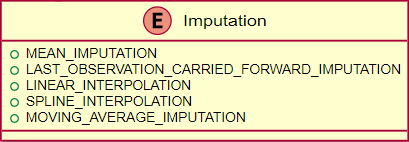
\includegraphics[width=4.5cm]{classes/model-management/5.png}}
\end{wrapfigure} 
\par
This class is blablabla and bla bla bla. This denotes bla bla bla and provided by Selehaddin Ozdemir. xdaslkads anu adl kl;asd k;lads l;l;kasdk ;lkdsa;k lllld kksdk mjdask hdaksjhd haso sadjh salk da.
\newline
\newline

\subsubsection{Feature}
\label{Feature}
\begin{wrapfigure}{l}{4.5cm}
    \raisebox{0pt}[\dimexpr\height-0.5\baselineskip\relax]{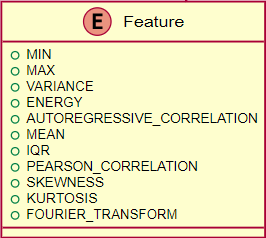
\includegraphics[width=4.5cm]{classes/model-management/6.png}}
\end{wrapfigure} 
\par
This class is blablabla and bla bla bla. This denotes bla bla bla and provided by Selehaddin Ozdemir. xdaslkads anu adl kl;asd k;lads l;l;kasdk ;lkdsa;k lllld kksdk mjdask hdaksjhd haso sadjh salk da.
\newline
\newline
\newline
\newline

\subsubsection{Normalizer}
\label{Normalizer}
\begin{wrapfigure}{l}{4.5cm}
    \raisebox{0pt}[\dimexpr\height-0.5\baselineskip\relax]{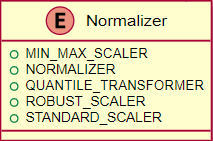
\includegraphics[width=4.5cm]{classes/model-management/7.png}}
\end{wrapfigure} 
\par
This class is blablabla and bla bla bla. This denotes bla bla bla and provided by Selehaddin Ozdemir. xdaslkads anu adl kl;asd k;lads l;l;kasdk ;lkdsa;k lllld kksdk mjdask hdaksjhd haso sadjh salk da.
\newline
\newline

\subsubsection{Factory}
\label{Factory}
\begin{wrapfigure}{l}{4.5cm}
    \raisebox{0pt}[\dimexpr\height-0.5\baselineskip\relax]{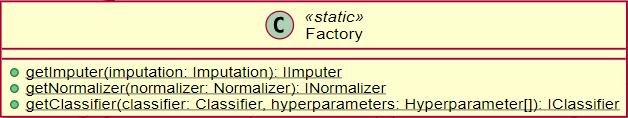
\includegraphics[width=4.5cm]{classes/model-management/8.png}}
\end{wrapfigure} 
\par
This static class is responsible for creating imputer, normalizer and classifier objects.
\newline
\newline
\textbf{Methods}
\begin{itemize}
    \item \textbf{getImputer} creates and returns an imputer object with the given name of the imputer
    \item \textbf{getNormalizer} creates and returns a normalizer object with the given name of the normalizer
    \item \textbf{getClassifier} creates and returns a classifier object with the given name of the classifier
\end{itemize}

\subsubsection{IImputer}
\label{IImputer}
\begin{wrapfigure}{l}{4.5cm}
    \raisebox{0pt}[\dimexpr\height-0.5\baselineskip\relax]{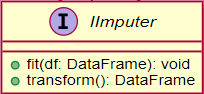
\includegraphics[width=4.5cm]{classes/model-management/9.png}}
\end{wrapfigure} 
\par
This is an interface for an imputer object.
\newline
\newline
\textbf{Methods}
\begin{itemize}
    \item \textbf{fit} fits the given data in the imputer object
    \item \textbf{transform} imputes the given data
\end{itemize}

\subsubsection{INormalizer}
\label{INormalizer}
\begin{wrapfigure}{l}{4.5cm}
    \raisebox{0pt}[\dimexpr\height-0.5\baselineskip\relax]{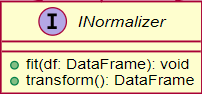
\includegraphics[width=4.5cm]{classes/model-management/10.png}}
\end{wrapfigure} 
\par
This is an interface for a normalizer object.
\newline
\newline
\textbf{Methods}
\begin{itemize}
    \item \textbf{fit} fits the given data in the normalizer object
    \item \textbf{transform} normalizes the given data
\end{itemize}

\subsubsection{IClassifier}
\label{IClassifier}
\begin{wrapfigure}{l}{4.5cm}
    \raisebox{0pt}[\dimexpr\height-0.5\baselineskip\relax]{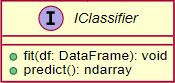
\includegraphics[width=4.5cm]{classes/model-management/11.png}}
\end{wrapfigure} 
\par
This is an interface for a classifier object.
\newline
\newline
\textbf{Methods}
\begin{itemize}
    \item \textbf{fit} fits the given data in the classifier object
    \item \textbf{predict} predicts of which label this data is
\end{itemize}

\subsubsection{PerfomanceMetrics}
\label{PerformanceMetrics}
\begin{wrapfigure}{l}{4.5cm}
    \raisebox{0pt}[\dimexpr\height-0.5\baselineskip\relax]{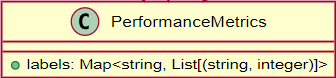
\includegraphics[width=4.5cm]{classes/model-management/12.png}}
\end{wrapfigure} 
\par
This class represents the performance metrics of a trained model.
\newline
\newline
\textbf{Attributes}
\begin{itemize}
    \item \textbf{labels} map of labels to their performance metrics
\end{itemize}

\subsubsection{Hyperparameter}
\label{Hyperparameter}
\begin{wrapfigure}{l}{4.5cm}
    \raisebox{0pt}[\dimexpr\height-0.5\baselineskip\relax]{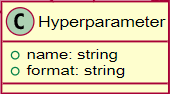
\includegraphics[width=4.5cm]{classes/model-management/13.png}}
\end{wrapfigure} 
\par
This class represents a hyperparameter for training a model.
\newline
\newline
\textbf{Attributes}
\begin{itemize}
    \item \textbf{name} name of the hyperparameter
    \item \textbf{format} the format of the value that the hyperparameter can get
\end{itemize}

\subsubsection{WorkspaceData}
\label{WorkspaceData}
\begin{wrapfigure}{l}{4.5cm}
    \raisebox{0pt}[\dimexpr\height-0.5\baselineskip\relax]{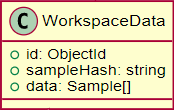
\includegraphics[width=4.5cm]{classes/model-management/14.png}}
\end{wrapfigure} 
\par
This class holds the sample data from the last training.
\newline
\newline
\textbf{Attributes}
\begin{itemize}
    \item \textbf{sampleHash} hash of the sample data
    \item \textbf{data} the sample data
\end{itemize}

\subsubsection{SlidingWindow}
\label{SlidingWindow}
\begin{wrapfigure}{l}{4.5cm}
    \raisebox{0pt}[\dimexpr\height-0.5\baselineskip\relax]{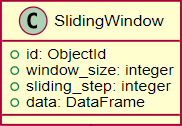
\includegraphics[width=4.5cm]{classes/model-management/15.png}}
\end{wrapfigure} 
\par
This class hold the sample data from recent trainings which is split into windows.
\newline
\newline
\textbf{Attributes}
\begin{itemize}
    \item \textbf{window\_size} size of the windows
    \item \textbf{sliding\_step} the sliding step of the windows
    \item \textbf{data} the sliding windows
\end{itemize}

\subsubsection{ImputedData}
\label{ImputedData}
\begin{wrapfigure}{l}{4.5cm}
    \raisebox{0pt}[\dimexpr\height-0.5\baselineskip\relax]{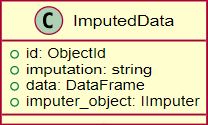
\includegraphics[width=4.5cm]{classes/model-management/16.png}}
\end{wrapfigure} 
\par
This class holds the imputed data from recent trainings.
\newline
\newline
\textbf{Attributes}
\begin{itemize}
    \item \textbf{imputation} the used imputation method
    \item \textbf{data} the imputed data
    \item \textbf{imputer\_object} the used imputer object
\end{itemize}

\subsubsection{ExtractedFeature}
\label{ExtractedFeature}
\begin{wrapfigure}{l}{4.5cm}
    \raisebox{0pt}[\dimexpr\height-0.5\baselineskip\relax]{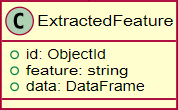
\includegraphics[width=4.5cm]{classes/model-management/17.png}}
\end{wrapfigure} 
\par
This class holds the extracted features of the data from recent trainings.
\newline
\newline
\textbf{Attributes}
\begin{itemize}
    \item \textbf{feature} the extracted feature
    \item \textbf{data} the values of the feature
\end{itemize}

\newpage
\section{Sequence Diagrams}

\subsection{General Sequence}
This sequence diagram shows the interaction between the components of the system via the API calls.
\begin{figure}[!htb]
    \centering
    \fbox{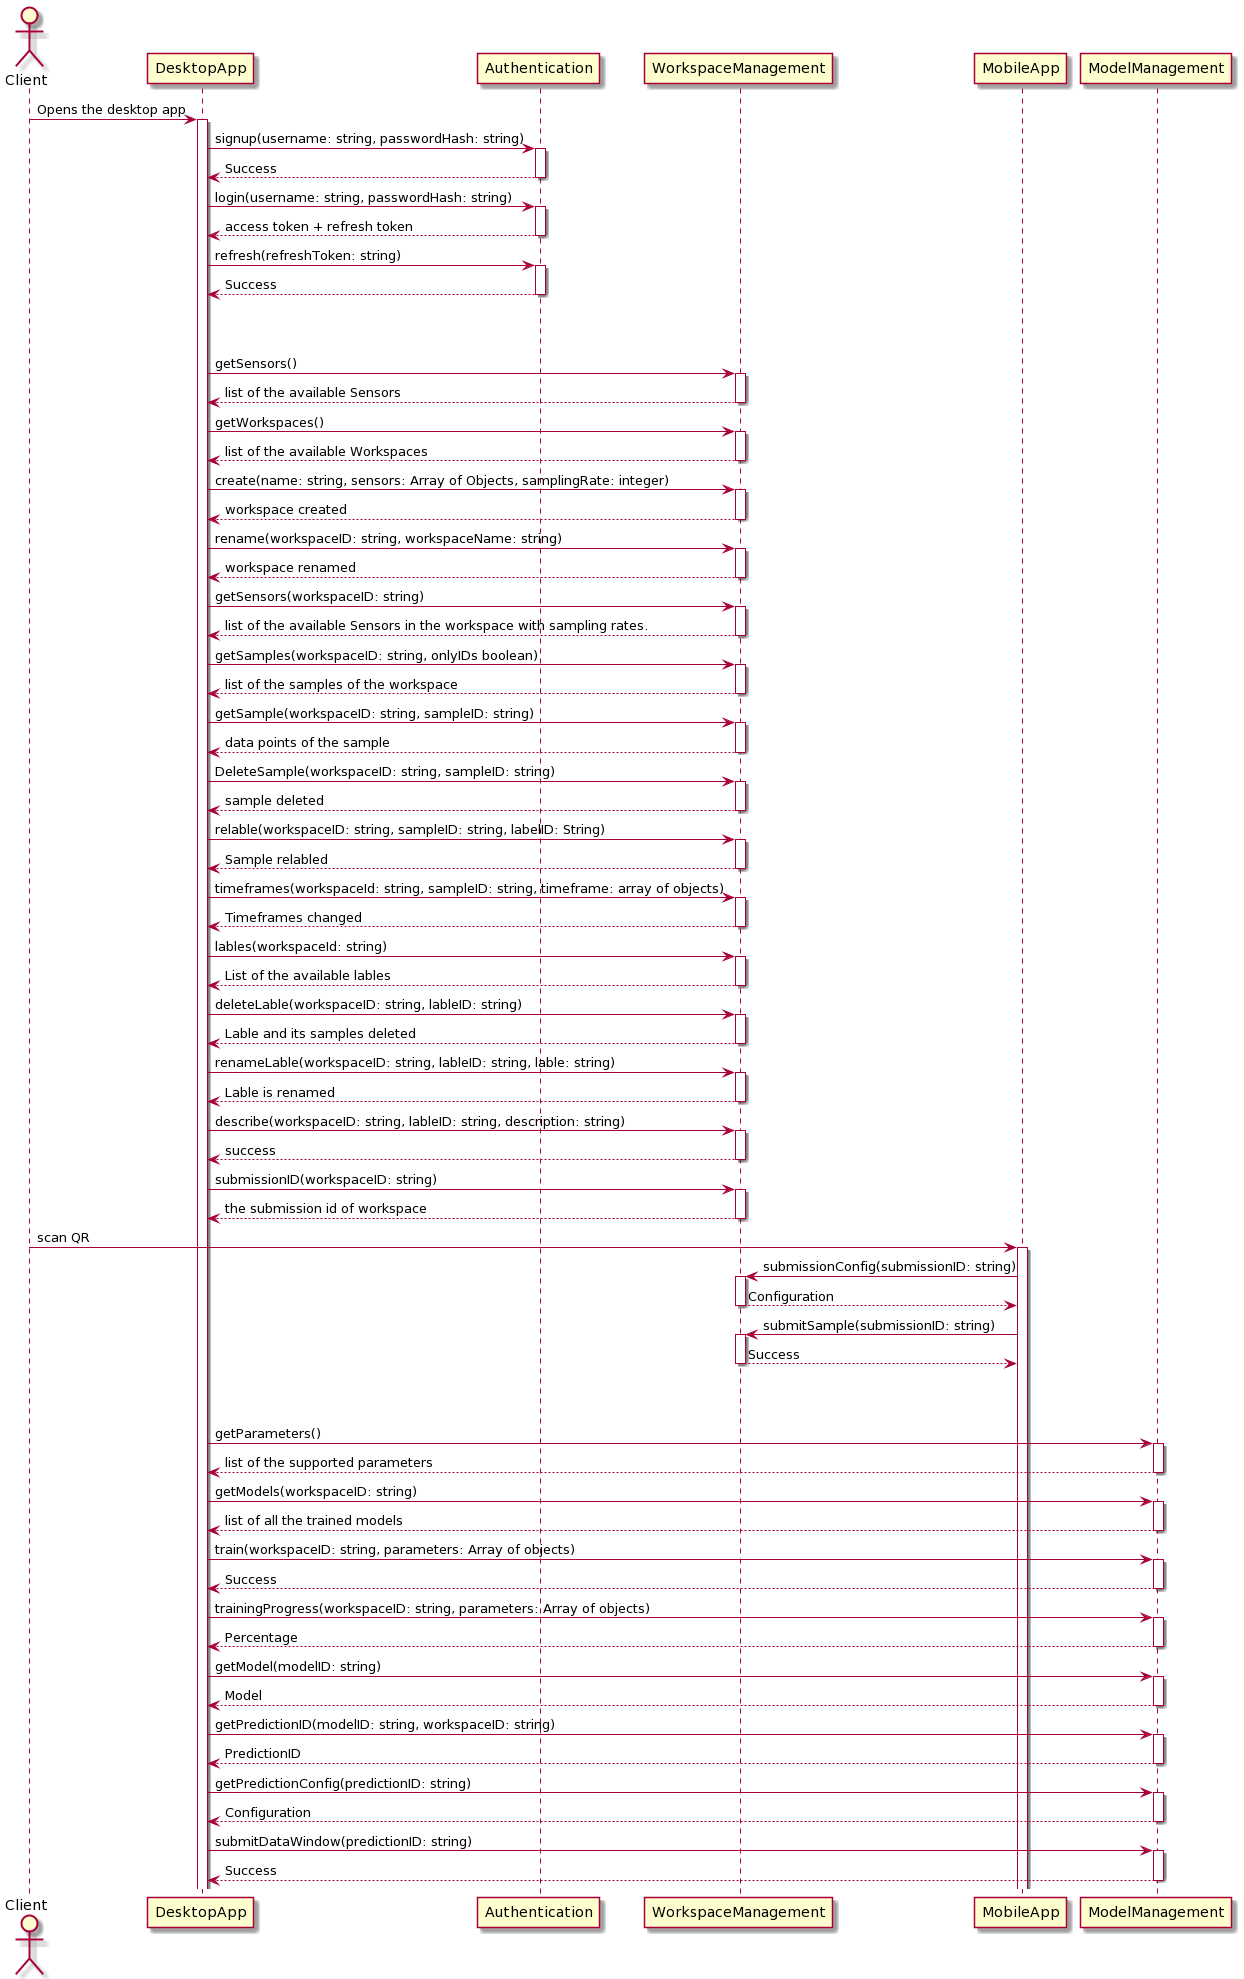
\includegraphics[width = .98\textwidth, height = .80\textheight]{figures/seq-general.png}}
    \caption{General Sequence}
    \label{fig:seq-general}
\end{figure}

\subsection{Desktop Client}

\subsubsection{Authentication}
\begin{figure}[hb]
    \centering
    \fbox{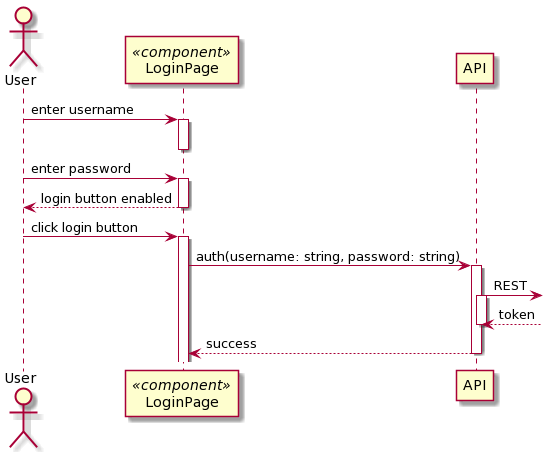
\includegraphics[width = .98\textwidth]{figures/seq-desktop-auth.png}}
    \caption{Authentication Sequence}
    \label{fig:seq-desktop-auth}
\end{figure}

\textbf{explanation}
\newpage

\subsubsection{Workspace Creation}
\begin{figure}[!htb]
    \centering
    \fbox{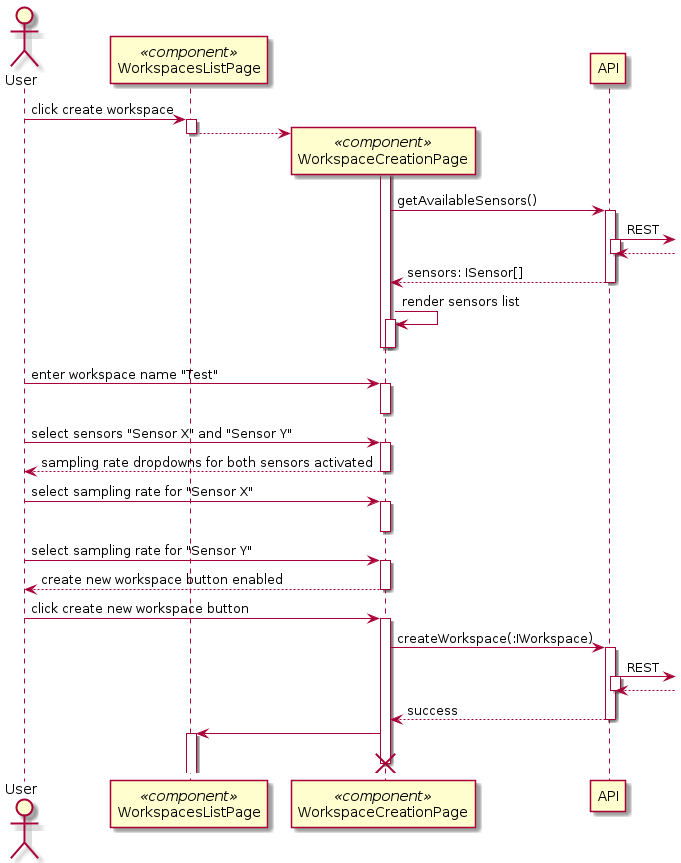
\includegraphics[width = .98\textwidth]{figures/seq-desktop-workspace-create.png}}
    \caption{Workspace Creation Sequence}
    \label{fig:seq-desktop-workspace-create}
\end{figure}

\textbf{explanation}
\newpage

\subsubsection{Timeframing a Sample}
\begin{figure}[!htb]
    \centering
    \fbox{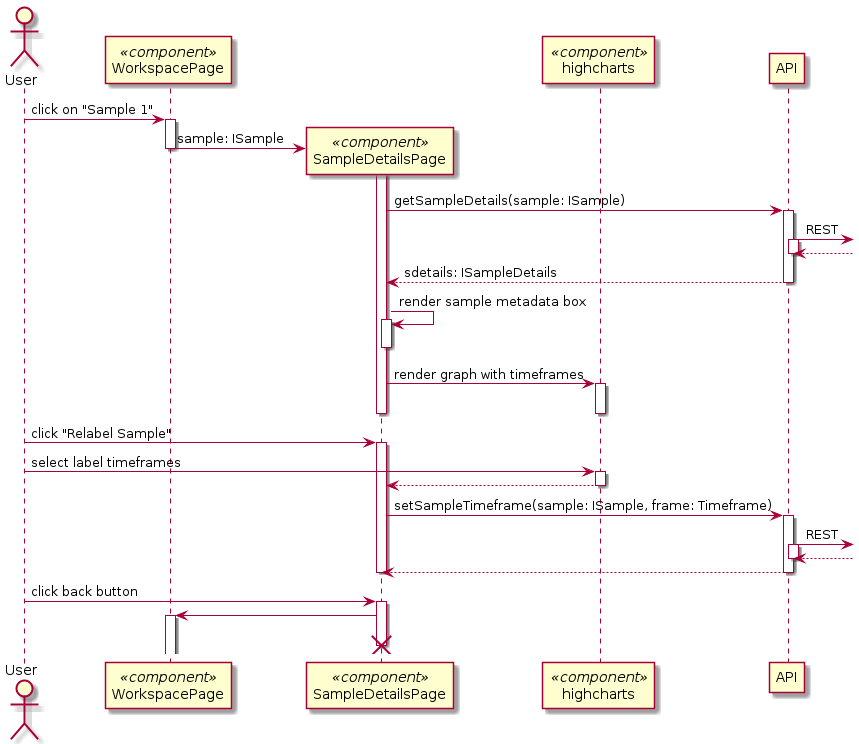
\includegraphics[width = .98\textwidth]{figures/seq-timeframing-a-sample.png}}
    \caption{Sample Timeframing Sequence}
    \label{fig:seq-timeframing-a-sample}
\end{figure}

\textbf{explanation}
\newpage

\subsection{Mobile Client}

\subsection{Authentication}

This diagram shows the registration and validation process of new user accounts. The user first registers with his email, username and a password of his choice and then receives an email that has a validation code. The user enters this token to the desktop client and validates his account.
\subsubsection{Registration and Validation}
\begin{figure}[!htb]
    \centering
    \fbox{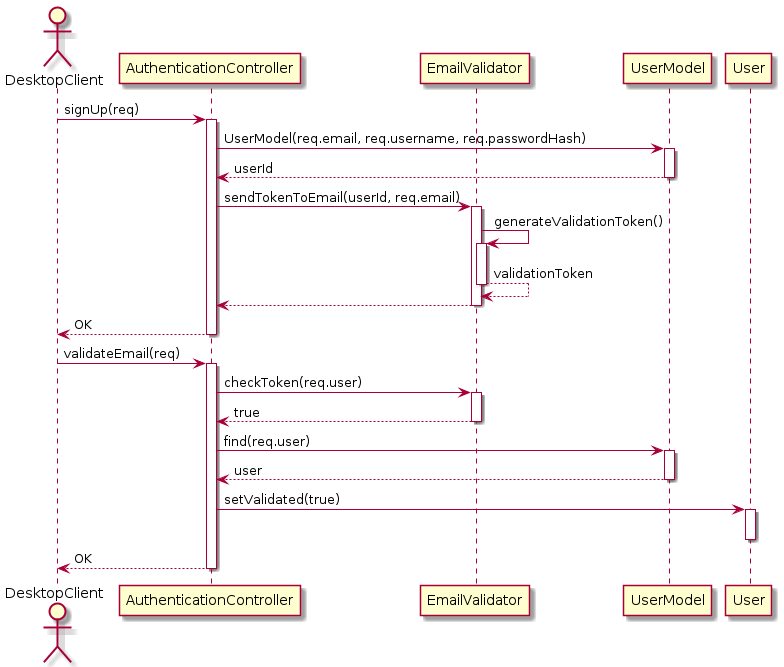
\includegraphics[width = 0.98\textwidth, height = 0.78\textheight]{figures/seq-auth-register-and-validate.png}}
    \caption{Registration and Validation}
    \label{fig:seq-auth-register-and-validate}
\end{figure}

\subsubsection{Login}
This diagram shows the login process. The user has already created an account and logs in. The received token is valid for a set amount of time which is then refresh by another token.
\begin{figure}[!htb]
    \centering
    \fbox{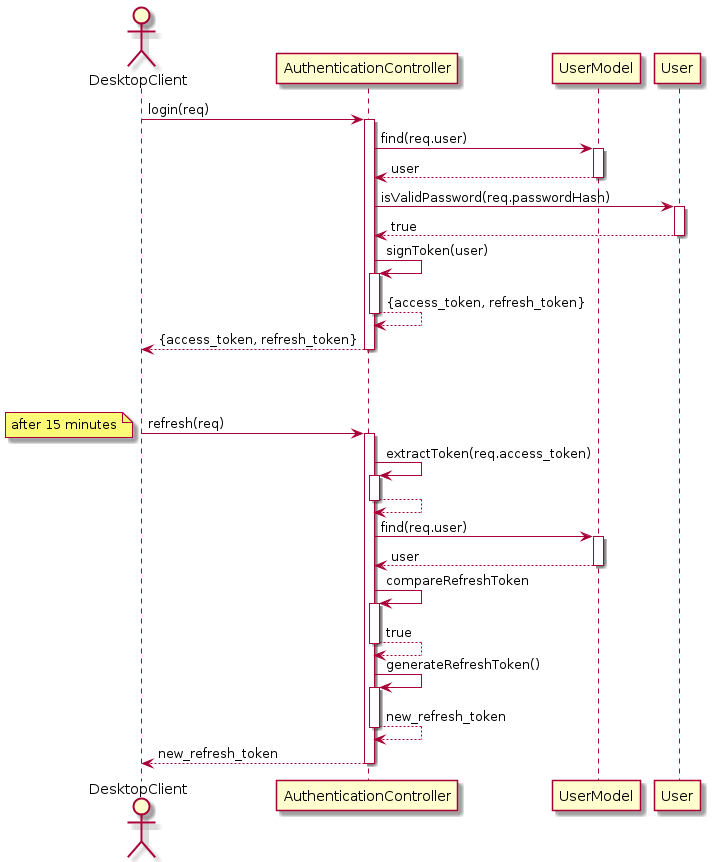
\includegraphics[width = 0.98\textwidth, height = 0.78\textheight]{figures/seq-auth-login.png}}
    \caption{Authentication Login}
    \label{fig:seq-auth-login}
\end{figure}

\subsection{Workspace Management}

\subsubsection{Create and Rename Workspace}
In this diagram, the user has no workspace initially. He then access the workspace creation tab of the desktop client. The desktop client asks the server which sensors are available as well as their default and maximum sampling rates. The user chooses the sensors he wishes to use and a name to his workspace. After creating it, the user renames the workspace.
\begin{figure}[!htb]
    \centering
    \fbox{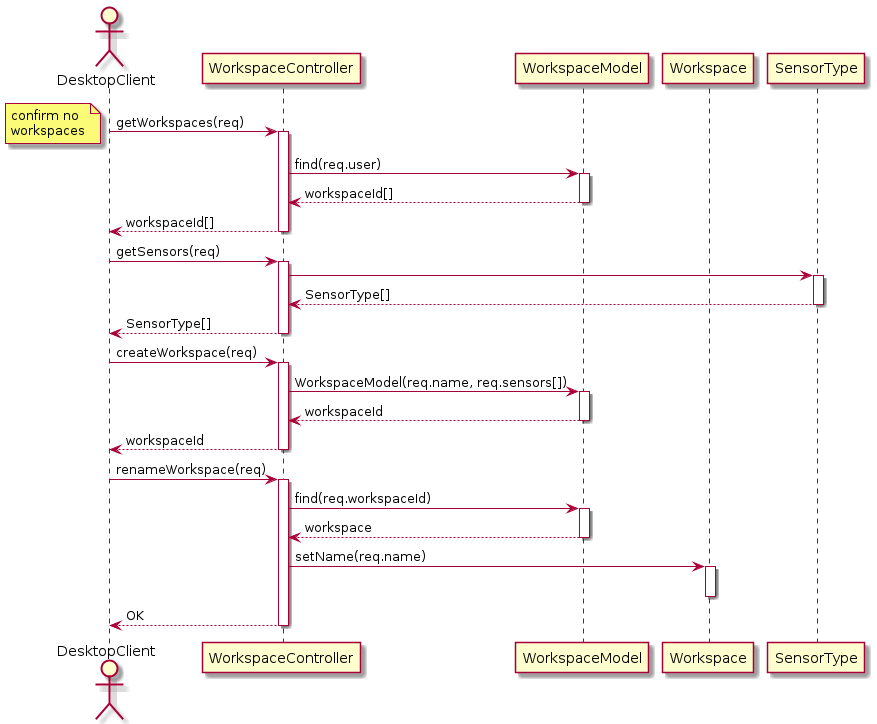
\includegraphics[width = 0.98\textwidth, height = 0.78\textheight]{figures/seq-workspace-create-and-rename.png}}
    \caption{Create and Rename}
    \label{fig:seq-workspace-create-and-rename}
\end{figure}
\newpage

\subsubsection{Submit Sample}
This diagram depicts the sample submission process. To start the sample collection, the desktop client asks for a submission id. After receiving the submission id, it embeds the id to a QR code which is scanned by the mobile client. The mobile client requests the submission config, i.e. which sensors are to be used for the recording and which labels are available. After the recording concludes, the sample is pushed to the server. A new entry for the sample is created in the server database.
\begin{figure}[!htb]
    \centering
    \fbox{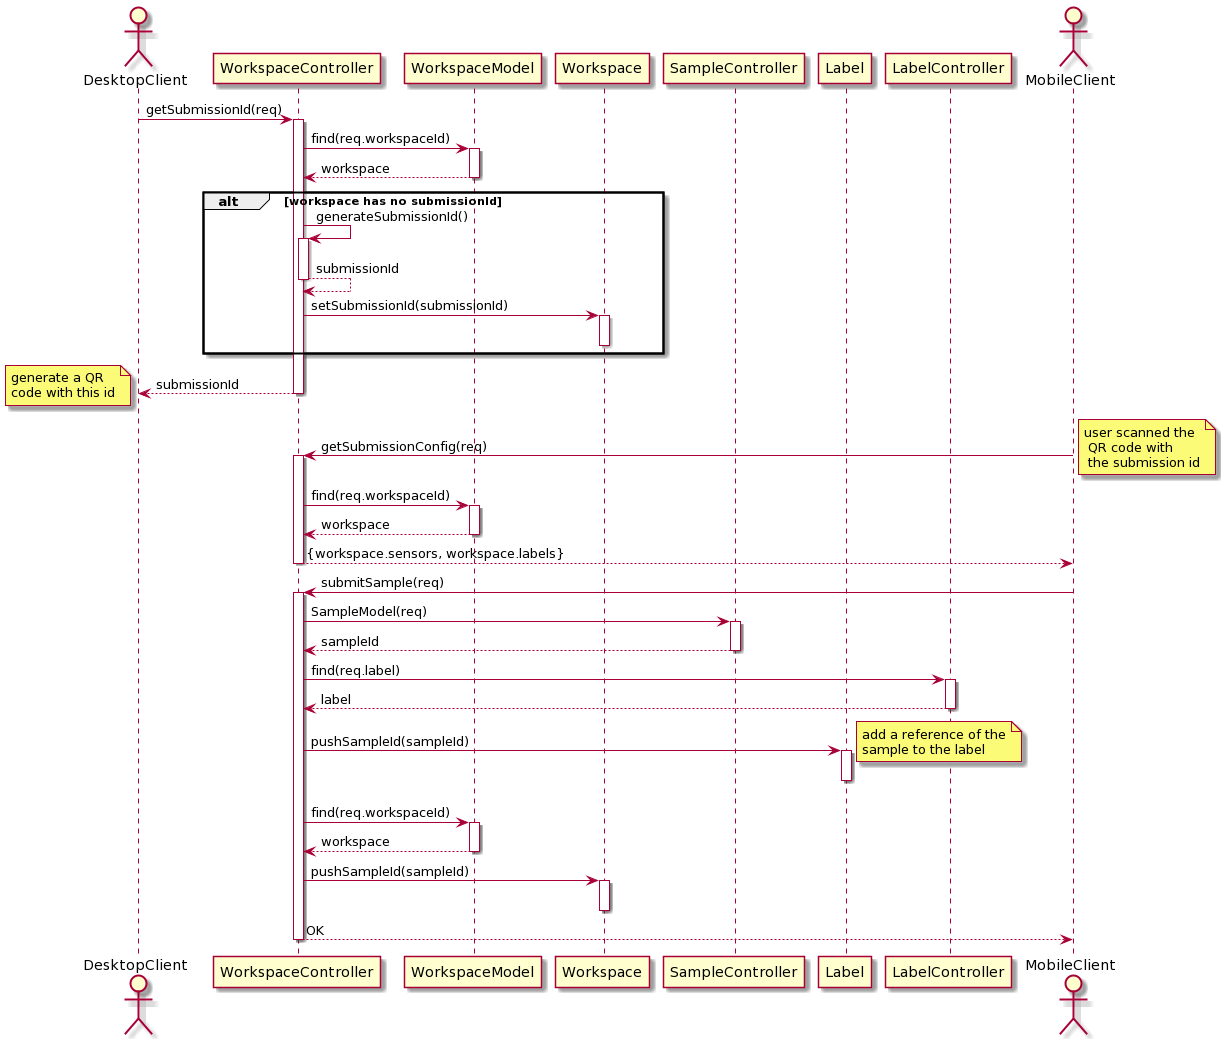
\includegraphics[width = 0.98\textwidth, height = 0.78\textheight]{figures/seq-workspace-submit-data.png}}
    \caption{Submit Data}
    \label{fig:seq-workspace-submit-data}
\end{figure}

\subsubsection{Create, Add Description and Delete Labels}
In this diagram, the user creates a new label to use for his samples by choosing a name. He then adds a description to the label. After that, he deletes a label from the workspace which in turn deletes all the samples in the workspace with that label.
\begin{figure}[!htb]
    \centering
    \fbox{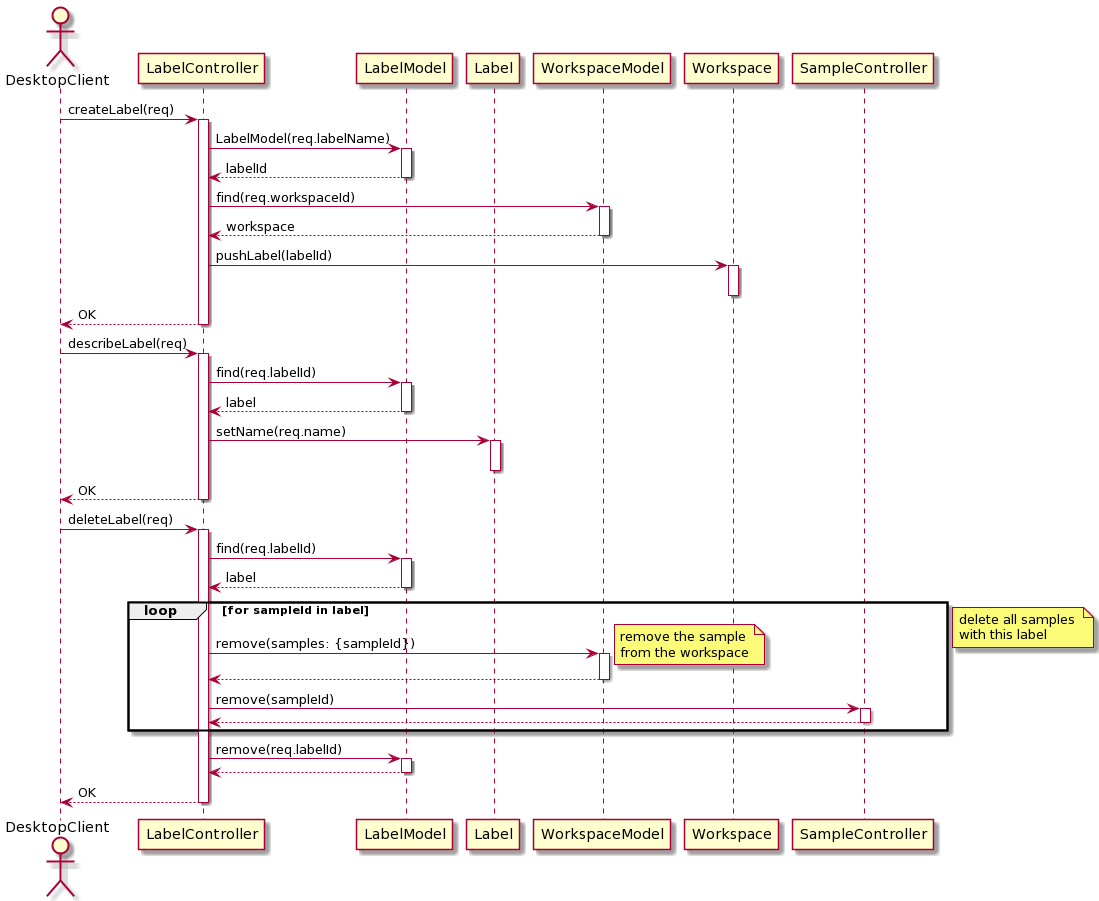
\includegraphics[width = 0.98\textwidth, height = 0.78\textheight]{figures/seq-workspace-management.png}}
    \caption{General Workspace Management}
    \label{fig:seq-workspace-management}
\end{figure}

\subsection{Model Management}

\subsubsection{Training a Model}
This sequence diagram shows how a train request is handled in the Model Management Server. In the beginning, a database connection is established, a Router instance is created, and a new workspace is created with the createModelWorkspace request from the Workspace Management Server.
The user first requests all the available training parameters with the getParameters request. Then the user requests training a model with the given name and training parameters. The model training is done in a Trainer instance. The training can be seen as a pipeline with the following parts: Retrieving samples, splitting to windows, imputation, feature extraction, normalization, classification and storing the new model in the database. The results of the steps from retrieving samples to feature extraction from recent model trainings are stored in the database, and they can be used if the samples or the parameters haven't changed. At the end, the created imputer, normalizer and classifier objects as well as its performance metrics are stored in the new MLModel instance and then stored in the database.
\begin{figure}[!htb]
    \centering
    \fbox{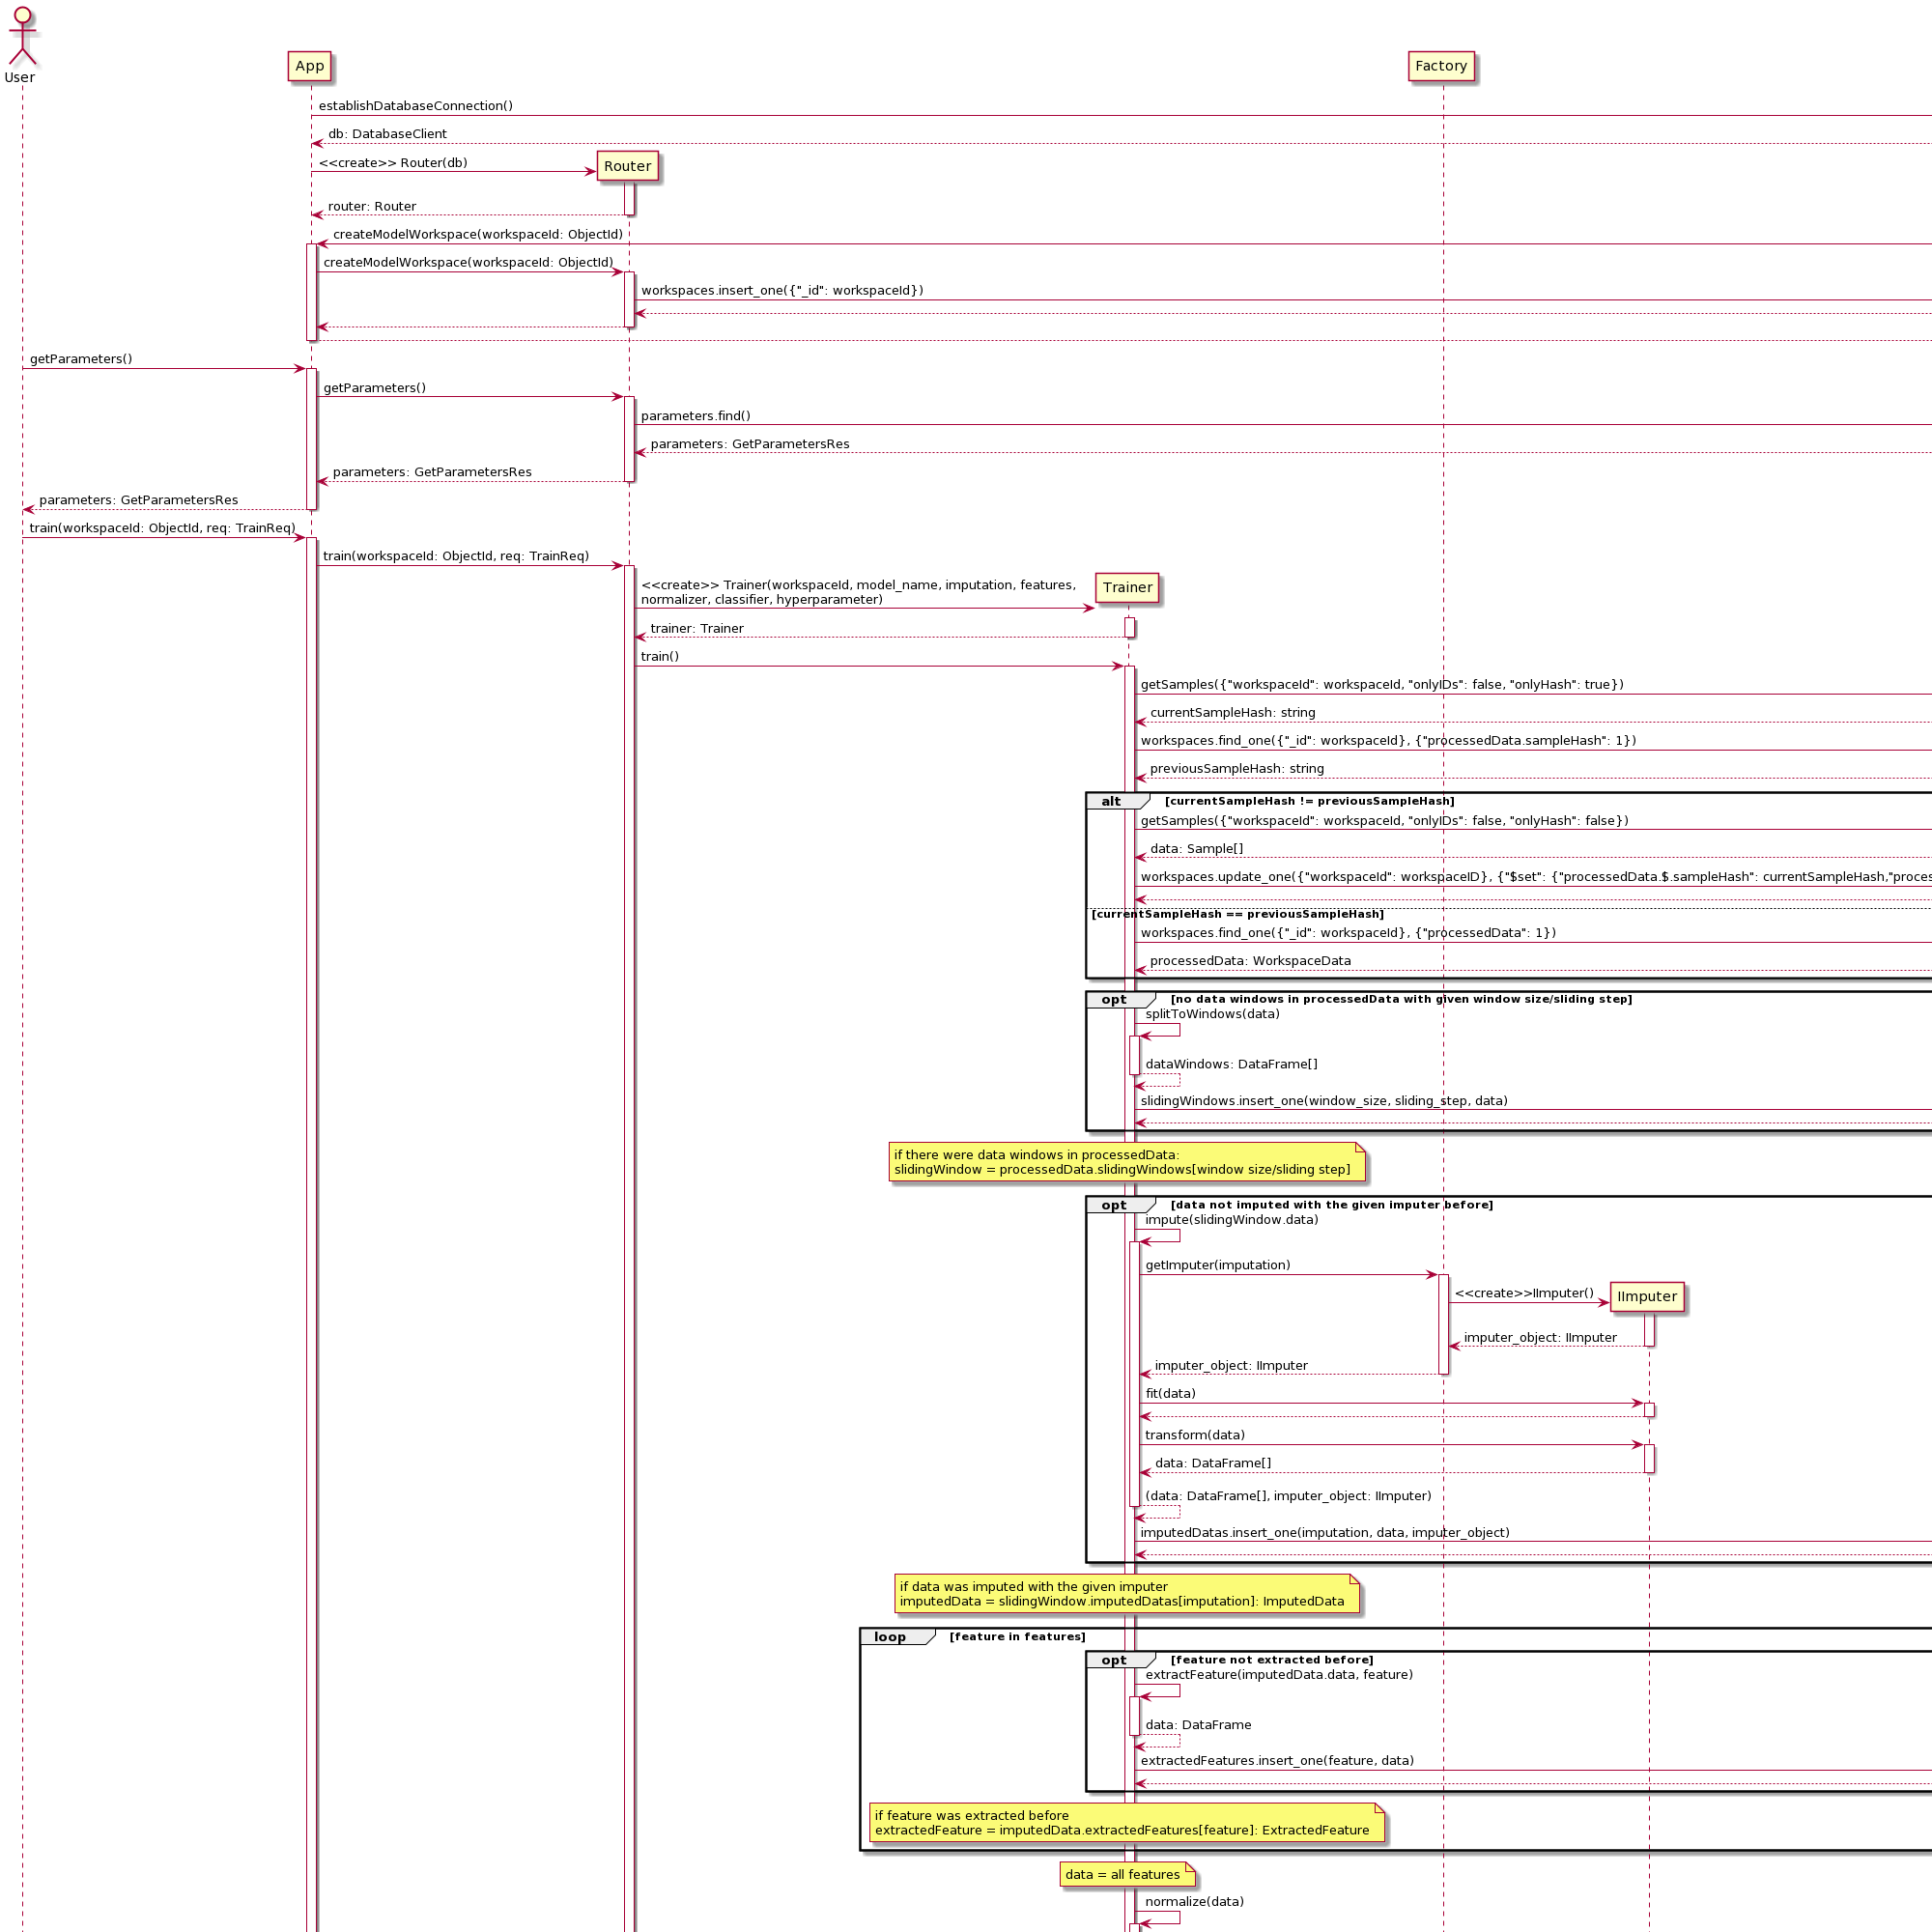
\includegraphics[width = 0.98\textwidth, height = 0.85\textheight]{figures/seq-training-a-model.png}}
    \caption{Model Training Sequence}
    \label{fig:seq-training-a-model}
\end{figure}


\subsubsection{Prediction}
In this sequence diagram, a user uses one of the trained models to classify his actions with his mobile. At first, the user gets all the IDs of the models and chooses the model which the user wants to use. The user then gets a prediction ID of this model, which is embedded in a QR code. When scanned, the mobile client requests the prediction configuration of this model, which returns the sensors to be used and their sampling rates. A new Predictor instance is created in the backend with the imputer, normalizer and classifier object of the model as well as the labels of the workspace. As long as the user submits data, the trainer does the needed imputation, feature extraction and normalization of the data. The classifier object then predicts the data. The trainer class counts the number of times the labels were predicted. When the getPrediction request is called, the label with the highest count of predictions is returned, and the counters are reset.
\begin{figure}[!htb]
    \centering
    \fbox{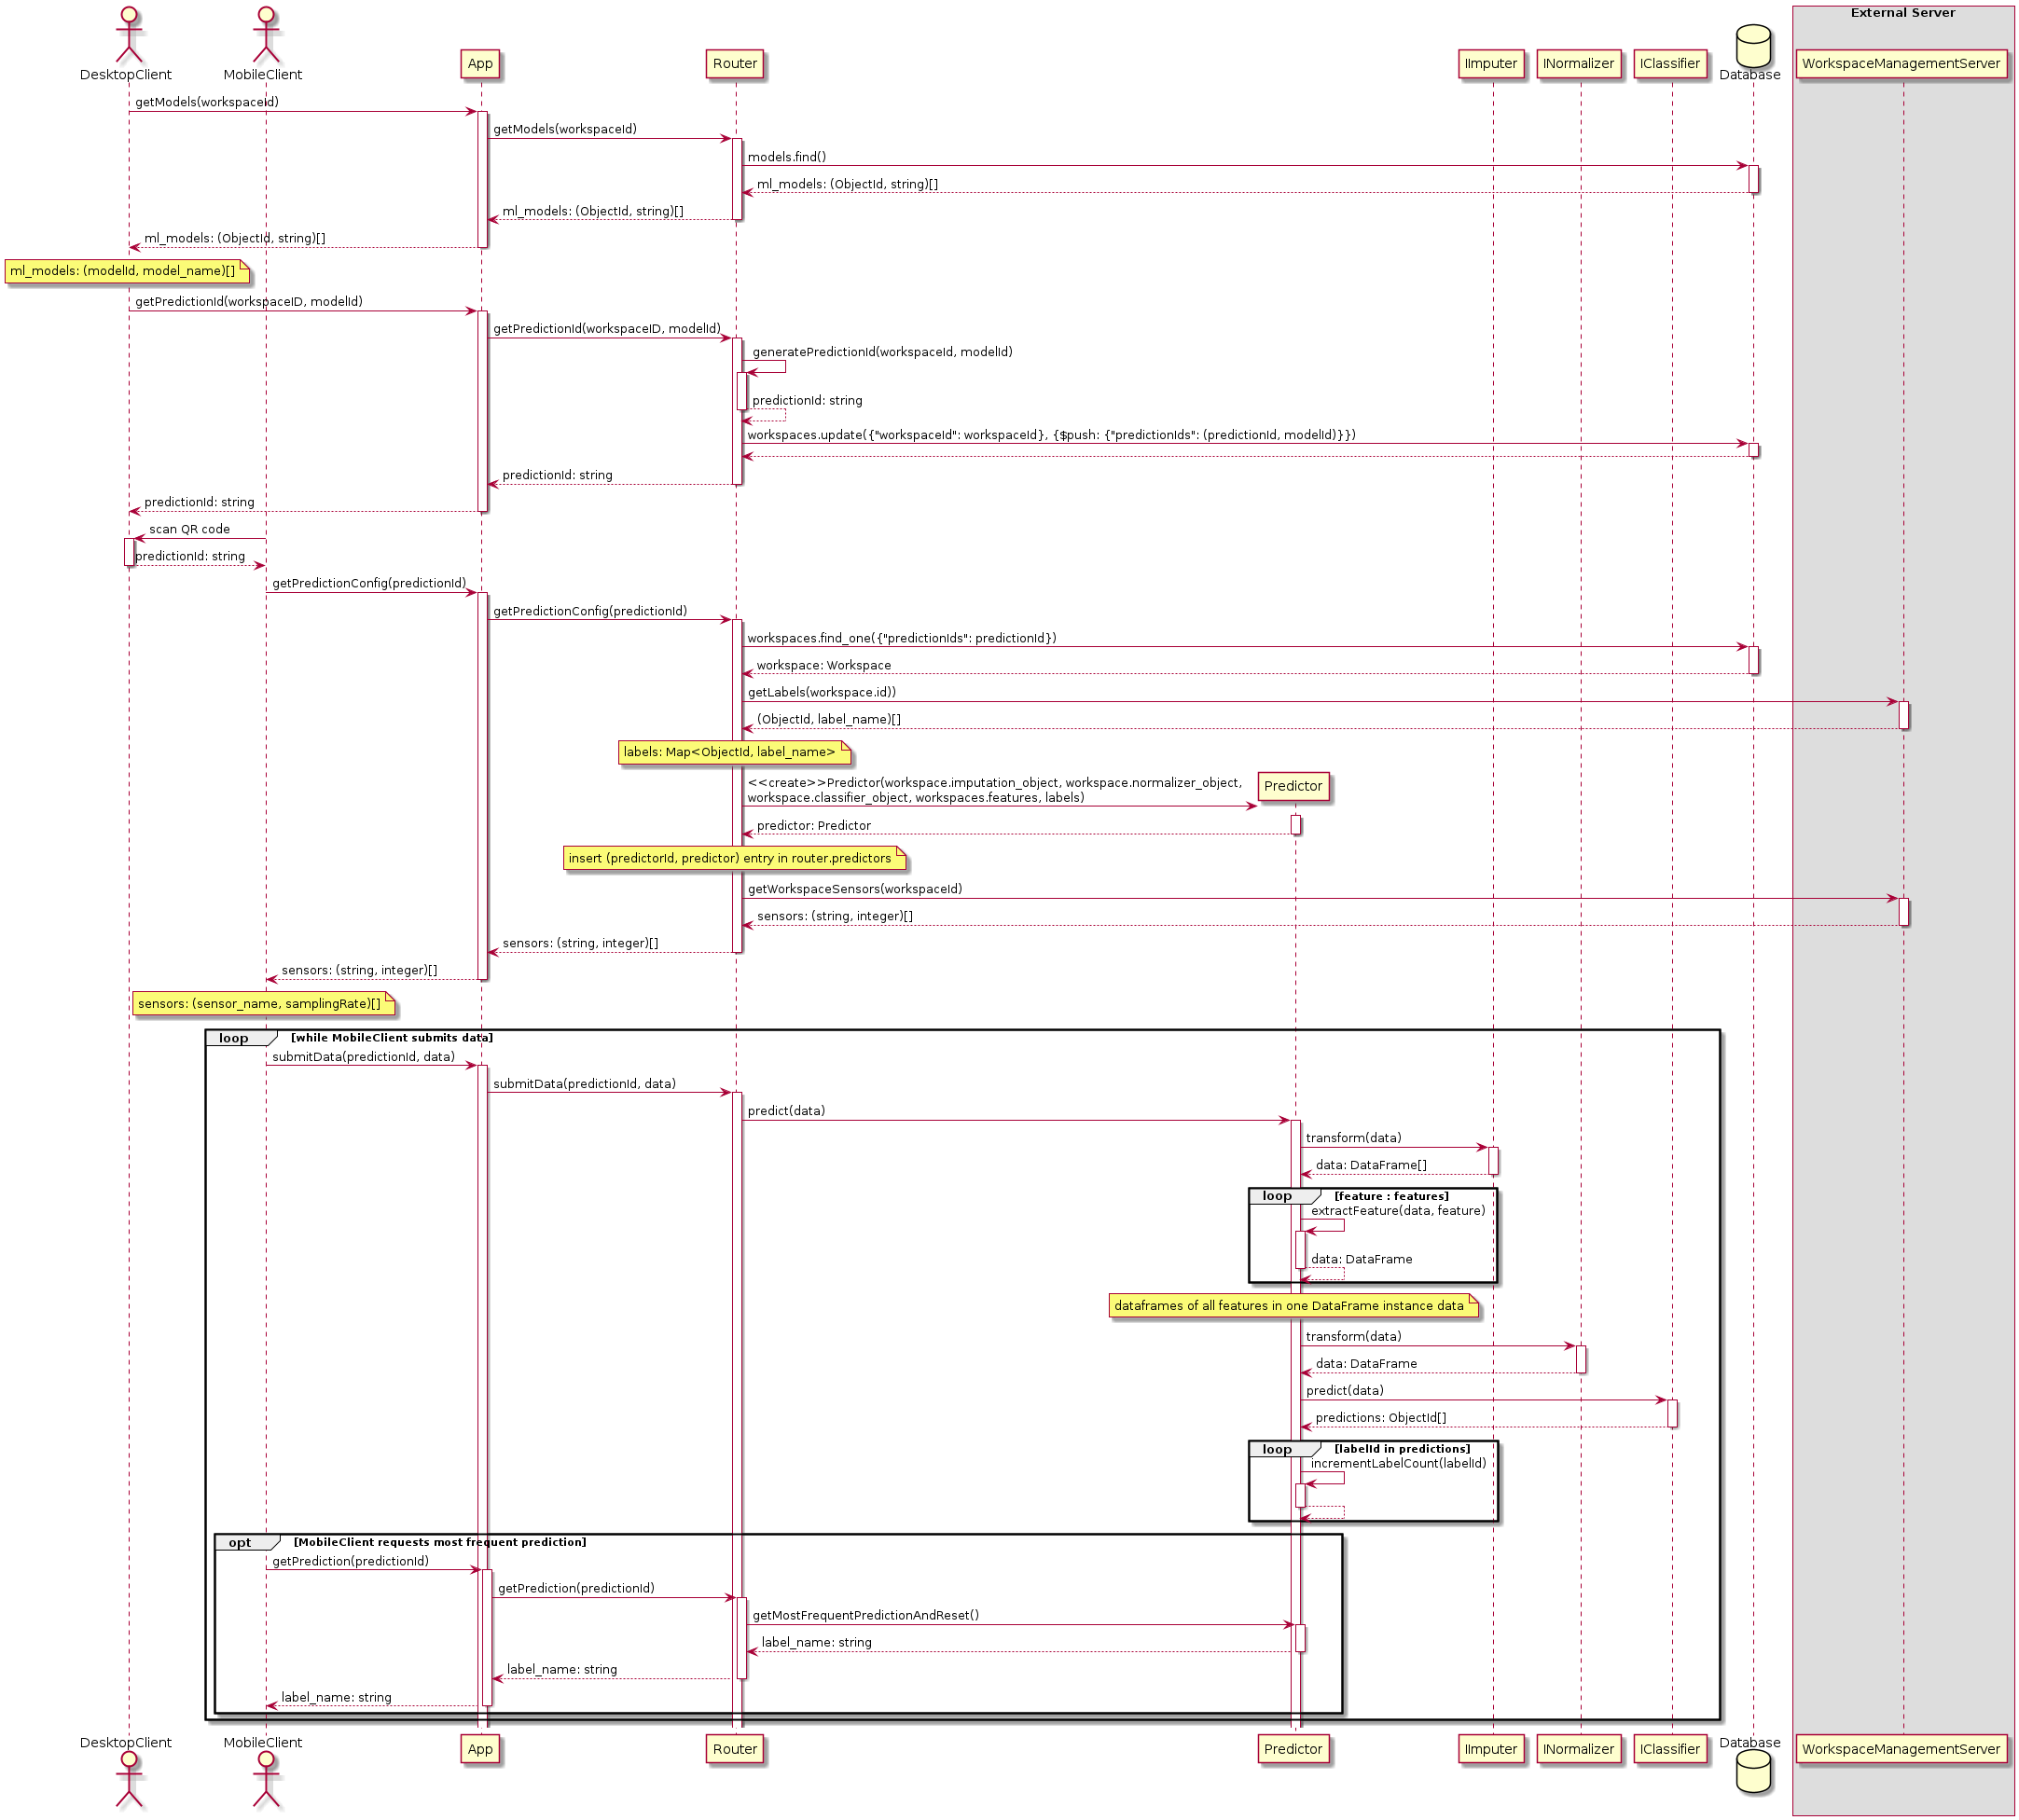
\includegraphics[width = 0.98\textwidth, height = 0.80\textheight]{figures/seq-predict.png}}
    \caption{Mobile Prediction Sequence}
    \label{fig:seq-predict}
\end{figure}

\textbf{explanation}
\newpage
\section{Design Data}
TBD

\newpage
\section{Class Index}

\subsection{Authentication}
\begin{itemize}
    \item \hyperref[App]{App}
    \item \hyperref[UserModel]{UserModel}
    \item \hyperref[User]{User}
    \item \hyperref[EmailValidator]{EmailValidator}
    \item \hyperref[TokenContent]{TokenContent}
\end{itemize}

\subsection{Workspace Management}
\begin{itemize}
    \item \hyperref[WorkspaceModel]{WorkspaceModel}
    \item \hyperref[wm-Workspace]{Workspace}
    \item \hyperref[SensorType]{SensorType}
    \item \hyperref[Sensor]{Sensor}
    \item \hyperref[Label]{Label}
    \item \hyperref[SampleModel]{SampleModel}
    \item \hyperref[Sample]{Sample}
    \item \hyperref[SensorDataPoints]{SensorDataPoints}
    \item \hyperref[DataPoint]{DataPoint}
    \item \hyperref[TimeFrame]{TimeFrame}
\end{itemize}

\subsection{Model Management}
\begin{itemize}
    \item \hyperref[Trainer]{Trainer}
    \item \hyperref[mm-Workspace]{Workspace}
    \item \hyperref[mm-Sensor]{Sensor}
    \item \hyperref[MLModel]{MLModel}
    \item \hyperref[Imputation]{Imputation}
    \item \hyperref[Feature]{Feature}
    \item \hyperref[Normalizer]{Normalizer}
    \item \hyperref[Factory]{Factory}
    \item \hyperref[IImputer]{IImputer}
    \item \hyperref[INormalizer]{INormalizer}
    \item \hyperref[IClassifier]{IClassifier}
    \item \hyperref[PerformanceMetrics]{PerformanceMetrics}
    \item \hyperref[Hyperparameter]{Hyperparameter}
    \item \hyperref[WorkspaceData]{WorkspaceData}
    \item \hyperref[SlidingWindow]{SlidingWindow}
    \item \hyperref[ImputedData]{ImputedData}
    \item \hyperref[ExtractedFeature]{ExtractedFeature}
\end{itemize}



\newpage
\section{Appendix}
Class diagrams are tiled in the next 36 pages. 


\printnoidxglossary

% END DOCUMENT
\end{document}
